\documentclass[11pt,letterpaper]{article}
\usepackage[margin=1in]{geometry}
\usepackage{graphicx}
\usepackage{amsmath}
\usepackage{amssymb}
\usepackage{hyperref}
\usepackage{booktabs}
\usepackage{xcolor}
\usepackage{enumitem}
\usepackage{caption}
\usepackage{multirow}
\usepackage[numbers,sort&compress]{natbib}

% Colors
\definecolor{darkblue}{RGB}{0,51,102}
\definecolor{darkred}{RGB}{153,0,0}
\definecolor{darkgreen}{RGB}{0,102,51}

\hypersetup{
    colorlinks=true,
    linkcolor=darkblue,
    citecolor=darkblue,
    urlcolor=darkblue
}

\title{\textbf{Physics-Informed Feature Engineering and Domain Shift Challenges for Atmospheric Machine Learning: Lessons from Cloud Base Height Retrieval}}

\author{
    Rylan Malarchick \\
    Embry-Riddle Aeronautical University \\
    Daytona Beach, FL 32114 \\
    \texttt{malarchr@my.erau.edu}
}

\date{February 2026 --- Iteration 2 (Audit Reconciled)}

\begin{document}

\maketitle

\begin{abstract}
We investigate physics-informed feature engineering and domain shift challenges for atmospheric machine learning, using cloud base height (CBH) retrieval as a case study. Starting from 5 base ERA5 reanalysis variables (t2m, d2m, sp, blh, tcwv), we derive 29 thermodynamic features grounded in cloud formation physics, including virtual temperature, stability-moisture interactions, and lifting condensation level variants, yielding 34 total features. More critically, we document catastrophic domain shift: leave-one-flight-out cross-validation across 5,500 ocean-only boundary-layer observations from six ER-2 flights yields R$^2$ = -5.36, indicating predictions worse than a constant baseline when generalizing across atmospheric regimes. This represents among the most severe domain shifts reported in atmospheric ML literature. We systematically evaluate five domain adaptation methods, finding that few-shot learning (50 samples) recovers R$^2$ = +0.35 while instance weighting and MMD alignment fail completely. Conformal prediction achieves only 34\% coverage (target: 90\%) due to exchangeability violations across flights, but within-flight calibration recovers 90\% coverage. Our findings establish that (1) physics-informed features provide interpretability advantages but limited accuracy gains over well-tuned base models, (2) domain shift is the critical challenge for atmospheric ML deployment, and (3) few-shot adaptation with 20--50 local samples is the most practical solution. We provide honest documentation of failure modes to guide practitioners toward realistic expectations for cross-regime generalization.
\end{abstract}

\textbf{Keywords:} domain adaptation, feature engineering, atmospheric machine learning, ERA5 reanalysis, conformal prediction, transfer learning

\section{Introduction}

\subsection{The Generalization Challenge in Atmospheric ML}

Machine learning has achieved remarkable success in atmospheric science applications, from precipitation nowcasting \cite{Rasp2020} to satellite retrieval algorithms \cite{Stubenrauch2021}. However, most studies report performance on held-out test sets drawn from the same distribution as training data. Real-world deployment faces a more challenging scenario: models trained on historical observations must generalize to new geographic regions, seasons, and atmospheric regimes never seen during training.

This paper investigates two interconnected challenges. The first concerns feature engineering: can physics-informed derived features improve predictions beyond raw reanalysis variables, and what thermodynamic relationships does the model learn? The second addresses domain shift: how severe is performance degradation when generalizing across atmospheric regimes, and what adaptation methods can recover performance?

We use cloud base height (CBH) retrieval from NASA ER-2 observations as a case study, but our findings have broad implications for any atmospheric ML application facing distribution shift between training and deployment.

\subsection{Contributions}

This work makes five key contributions. In the area of physics-based feature engineering, we derive 29 thermodynamic features from 5 base ERA5 variables, including virtual temperature, stability indices, and moisture-stability interactions, and analyze which features emerge as important and why. Regarding quantified domain shift, we document catastrophic generalization failure with R$^2$ = -5.36 across flight campaigns, characterize shift sources via K-S divergence and MMD analysis, and explain why standard cross-validation dramatically overestimates real-world performance. For domain adaptation evaluation, we systematically compare five adaptation methods including few-shot learning, instance weighting, TrAdaBoost, MMD alignment, and feature selection, identifying few-shot learning as the only effective approach. On uncertainty quantification under violation, we demonstrate that conformal prediction fails with only 34\% coverage when exchangeability assumptions are violated, and propose within-flight calibration achieving 90\% coverage. Finally, through honest failure documentation, we provide explicit guidance on when this approach works, when it fails, and what practitioners should expect for cross-regime deployment.

\subsection{Paper Organization}

Section~\ref{sec:background} reviews related work on feature engineering and domain adaptation. Section~\ref{sec:features} presents our physics-based feature derivation and importance analysis. Section~\ref{sec:domain_shift} quantifies domain shift and evaluates adaptation methods. Section~\ref{sec:uncertainty} addresses uncertainty quantification challenges. Section~\ref{sec:discussion} synthesizes findings into practical recommendations. Section~\ref{sec:conclusion} concludes.

\section{Background and Related Work}
\label{sec:background}

\subsection{Feature Engineering for Atmospheric Applications}

Traditional atmospheric retrieval algorithms rely heavily on physics-based features derived from domain knowledge \cite{Hersbach2020}. The lifting condensation level (LCL), computed from surface temperature and dewpoint, provides a first-order cloud base estimate based on parcel theory \cite{Lawrence2005}:

\begin{equation}
    \text{LCL} \approx 125 \times (T - T_d) \text{ meters}
\end{equation}

More sophisticated features capture atmospheric stability (potential temperature gradients), moisture availability (column water vapor, relative humidity), and thermodynamic interactions. The question is whether explicit feature engineering provides advantages over letting modern ML algorithms learn representations from raw variables.

\subsection{Domain Adaptation in Remote Sensing}

Domain shift---distribution mismatch between training and deployment data---is a fundamental challenge for remote sensing applications \cite{Tuia2016}. Atmospheric observations exhibit shift across multiple dimensions. Geographic regions present distinct challenges as tropical, polar, and continental regimes have fundamentally different thermodynamic characteristics. Seasonal variations manifest as summer convection patterns differ substantially from winter stratiform clouds. Instrumental factors including sensor degradation and calibration drift introduce additional sources of distribution mismatch.

Common adaptation approaches include instance reweighting \cite{Shimodaira2000}, domain-adversarial training \cite{Ganin2016}, and few-shot learning \cite{Finn2017}. However, applications to atmospheric science remain limited, with most studies assuming i.i.d. data splits.

\subsection{Conformal Prediction for Uncertainty Quantification}

Conformal prediction provides distribution-free prediction intervals with guaranteed coverage under exchangeability \cite{Shafer2008, Lei2018}:

\begin{equation}
    P(y \in [\hat{y} - q, \hat{y} + q]) \geq 1 - \alpha
\end{equation}

where $q$ is calibrated from held-out residuals. The key assumption is that calibration and test data are exchangeable---drawn from the same distribution in arbitrary order. This assumption is violated by temporal autocorrelation and domain shift, with consequences we quantify below.

\section{Physics-Based Feature Engineering}
\label{sec:features}

\subsection{Base ERA5 Features}

We extract 5 base features from ERA5 reanalysis \cite{Hersbach2020}, matched to CPL observation locations via nearest grid point and nearest hour:

\begin{table}[h]
    \centering
    \caption{Base ERA5 features for CBH prediction.}
    \label{tab:base_features}
    \begin{tabular}{lll}
        \toprule
        \textbf{Feature} & \textbf{Units} & \textbf{Physical Role} \\
        \midrule
        t2m (2m temperature) & K & Surface parcel energy \\
        d2m (2m dewpoint) & K & Surface moisture \\
        sp (surface pressure) & Pa & Altitude reference \\
        blh (boundary layer height) & m & Mixing depth \\
        tcwv (total column water) & kg/m$^2$ & Column moisture \\
        \bottomrule
    \end{tabular}
\end{table}

Solar zenith angle (SZA) and solar azimuth angle (SAA) are obtained from CPL geolocation fields; these are used in derived features (Section~\ref{sec:derived}) but are not ERA5 variables.

\subsection{Derived Thermodynamic Features}
\label{sec:derived}

We engineer 29 additional features grounded in cloud formation physics, for a total of 34 features (5 base ERA5 + 29 derived):

\subsubsection{LCL-Based Features (2)}

We derive two LCL-based features from the standard lifting condensation level approximation (LCL $\approx$ 125~$\times$~(T$_{2m}$ -- T$_d$)). The lcl feature provides the estimated cloud base from parcel theory. The lcl\_deficit (BLH~--~LCL) measures the relationship between boundary layer depth and expected cloud base, identifying when mixing extends above or below the condensation level.

\subsubsection{Thermodynamic Features (8)}

Eight thermodynamic features capture the atmospheric state relevant to cloud formation, as summarized in Table~\ref{tab:thermo_features}.

\begin{table}[h]
    \centering
    \caption{Derived thermodynamic features for CBH prediction.}
    \label{tab:thermo_features}
    \begin{tabular}{ll}
        \toprule
        \textbf{Feature} & \textbf{Physical Interpretation} \\
        \midrule
        t\_virtual & Temperature with moisture buoyancy effects \\
        dewpoint\_depression & Direct LCL driver (t2m -- d2m) \\
        rh & Surface relative humidity \\
        stability\_index & Atmospheric stratification ((t2m -- d2m) / 10) \\
        moisture\_gradient & Vertical moisture structure \\
        pressure\_altitude & Hypsometric altitude from surface pressure \\
        theta\_e & Equivalent potential temperature \\
        blh\_lcl\_ratio & Boundary layer height to LCL ratio \\
        \bottomrule
    \end{tabular}
\end{table}

Virtual temperature ($T_v$) is particularly important:
\begin{equation}
    T_v = T \times (1 + 0.61 \times w)
\end{equation}
where $w$ is mixing ratio (computed from dewpoint and surface pressure via the Clausius-Clapeyron relation). This captures how moisture affects air density and buoyancy, critical for convective cloud formation.

\subsubsection{Stability Features (4)}

Four stability features capture interaction effects between atmospheric stratification and moisture, as shown in Table~\ref{tab:stability_features}.

\begin{table}[h]
    \centering
    \caption{Derived stability features.}
    \label{tab:stability_features}
    \begin{tabular}{ll}
        \toprule
        \textbf{Feature} & \textbf{Formulation} \\
        \midrule
        stability\_tcwv & Stability index $\times$ total column water vapor \\
        dd\_blh & Dewpoint depression $\times$ BLH / 1000 \\
        t2m\_d2m\_ratio & Temperature to dewpoint ratio \\
        inversion\_strength & BLH $\times$ stability index \\
        \bottomrule
    \end{tabular}
\end{table}

These interaction terms capture how atmospheric stratification modulates moisture effects on cloud formation.

\subsubsection{Solar/Temporal Features (7)}

Seven solar and temporal features encode diurnal and geometric effects, as shown in Table~\ref{tab:solar_features}.

\begin{table}[h]
    \centering
    \caption{Derived solar and temporal features.}
    \label{tab:solar_features}
    \begin{tabular}{ll}
        \toprule
        \textbf{Feature} & \textbf{Description} \\
        \midrule
        sza\_cos, sza\_sin & Trigonometric solar zenith encoding \\
        saa\_cos, saa\_sin & Trigonometric solar azimuth encoding \\
        solar\_heating\_proxy & Estimated surface heating from geometry \\
        hour\_sin, hour\_cos & Diurnal cycle encoding \\
        \bottomrule
    \end{tabular}
\end{table}

\subsubsection{Interaction Features (8)}

Eight interaction features capture nonlinear relationships between base variables, as summarized in Table~\ref{tab:interaction_features}.

\begin{table}[h]
    \centering
    \caption{Derived interaction features.}
    \label{tab:interaction_features}
    \begin{tabular}{ll}
        \toprule
        \textbf{Feature} & \textbf{Interaction Type} \\
        \midrule
        t2m\_tcwv & Temperature-moisture interaction \\
        rh\_blh & Humidity-boundary layer interaction \\
        lcl\_sq & Quadratic LCL term \\
        blh\_sq & Quadratic boundary layer term \\
        t2m\_sp & Temperature-pressure interaction \\
        lat\_abs & Absolute latitude (geographic proxy) \\
        lon\_abs & Absolute longitude (geographic proxy) \\
        lat\_lon & Latitude-longitude interaction \\
        \bottomrule
    \end{tabular}
\end{table}

\subsection{Feature Importance Analysis}

\subsubsection{Base Model (5 Features)}

GBDT trained on the 5 base ERA5 features identifies blh (boundary layer height) as overwhelmingly dominant:

\begin{table}[h]
    \centering
    \caption{Feature importance for base 5-feature ERA5 model (pooled training across all flights).}
    \label{tab:base_importance}
    \begin{tabular}{lc}
        \toprule
        \textbf{Feature} & \textbf{Importance (\%)} \\
        \midrule
        blh & 63.3 \\
        d2m & 11.2 \\
        sp & 10.9 \\
        tcwv & 10.3 \\
        t2m & 4.4 \\
        \bottomrule
    \end{tabular}
\end{table}

The blh dominance reflects boundary layer dynamics: cloud base height in the marine boundary layer is primarily constrained by the mixing depth, which GBDT captures directly from the boundary layer height variable.

\subsubsection{Enhanced Model (34 Features)}

With derived features, importance redistributes:

\begin{table}[h]
    \centering
    \caption{Feature importance for enhanced 34-feature model (pooled training across all flights).}
    \label{tab:enhanced_importance}
    \begin{tabular}{lc}
        \toprule
        \textbf{Feature} & \textbf{Importance (\%)} \\
        \midrule
        blh\_sq & 32.3 \\
        blh & 16.9 \\
        stability\_tcwv & 8.0 \\
        moisture\_gradient & 8.0 \\
        blh\_lcl\_ratio & 4.4 \\
        Others (29 features) & 30.4 \\
        \bottomrule
    \end{tabular}
\end{table}

Three key observations emerge from this analysis. First, blh-derived features dominate the enhanced model, with blh\_sq (quadratic boundary layer height) capturing nonlinear mixing effects and blh itself retaining importance, together accounting for nearly 50\% of total importance. Second, stability-moisture interaction emerges as the third most important feature, with the product stability\_index$\times$tcwv capturing how atmospheric stratification modulates moisture effects---a physically meaningful relationship. Third, the moisture gradient feature captures vertical moisture structure relevant to cloud formation, complementing the column-integrated tcwv measurement.

\subsubsection{Ablation Study}

Despite importance redistribution, removing individual features causes minimal performance degradation:

\begin{table}[h]
    \centering
    \caption{Ablation study: Impact of removing top features. ``Pooled CV'' is shuffled 5-fold CV across all flights; ``Per-flight CV'' is the mean of within-flight shuffled CV across flights (stricter, no cross-flight leakage).}
    \label{tab:ablation}
    \begin{tabular}{lccc}
        \toprule
        \textbf{Configuration} & \textbf{Pooled CV R$^2$} & \textbf{Per-Flight CV R$^2$} & \textbf{$\Delta$ Per-Flight} \\
        \midrule
        All 34 features & -2.053 & -0.505 & -- \\
        Remove blh\_sq & -2.290 & -0.610 & -0.105 \\
        Remove blh & -2.409 & -0.602 & -0.097 \\
        Remove stability\_tcwv & -2.483 & -0.800 & -0.295 \\
        Remove moisture\_gradient & -3.372 & -0.615 & -0.110 \\
        Remove blh\_lcl\_ratio & -2.371 & -0.578 & -0.073 \\
        Base 5 features only & -0.564 & -2.042 & -1.537 \\
        \bottomrule
    \end{tabular}
\end{table}

\textbf{Critical finding:} Individual feature removal causes modest degradation in per-flight CV (up to $\Delta$R$^2$ = -0.295 for stability\_tcwv), but dropping from 34 to 5 base features dramatically worsens per-flight performance ($\Delta$R$^2$ = -1.537). Interestingly, pooled CV shows the opposite pattern: base-5 features achieve better pooled CV (R$^2$ = -0.564) than 34 features (R$^2$ = -2.053), suggesting derived features may overfit to flight-specific patterns in the pooled setting while genuinely capturing generalizable structure within flights. Neither achieves positive R$^2$ due to inter-flight variability, confirming that domain shift---not feature engineering---is the dominant challenge.

This suggests gradient boosting effectively performs implicit feature engineering, learning nonlinear combinations of base variables that capture the same thermodynamic relationships we explicitly derived.

\subsection{Physical Plausibility Validation}

To verify the model learns physically consistent relationships, we evaluate against atmospheric constraints:

\begin{table}[h]
    \centering
    \caption{Physical constraint validation. CBH bounds apply to the training/test data (which are filtered to ocean-only BL clouds $\leq$2 km by construction). LOFO predictions may exceed these bounds due to domain shift.}
    \label{tab:physics}
    \begin{tabular}{lccc}
        \toprule
        \textbf{Constraint} & \textbf{Expected} & \textbf{Observed} & \textbf{Notes} \\
        \midrule
        Data CBH $\leq$ 2,000 m & 100\% & 100\% & Filtered by design \\
        Data CBH $>$ 0 m & 100\% & 100\% & Filtered by design \\
        LOFO pred $<$ 0 m & 0\% & 1.7\% & 91/5500 negative predictions \\
        \bottomrule
    \end{tabular}
\end{table}

The training data satisfies physical bounds by construction (ocean-only, BL clouds $\leq$ 2 km). However, 1.7\% of LOFO predictions are negative, a consequence of models trained on one atmospheric regime producing unphysical extrapolations when applied to a different regime---further evidence of the domain shift problem.

\section{Domain Shift and Adaptation}
\label{sec:domain_shift}

\subsection{Quantifying Domain Shift}

The fundamental challenge we document is catastrophic performance degradation when models trained on one atmospheric regime are applied to different conditions. Figure~\ref{fig:domain_comparison} illustrates the dramatic differences in cloud structure between the two campaigns.

\begin{figure}[h]
    \centering
    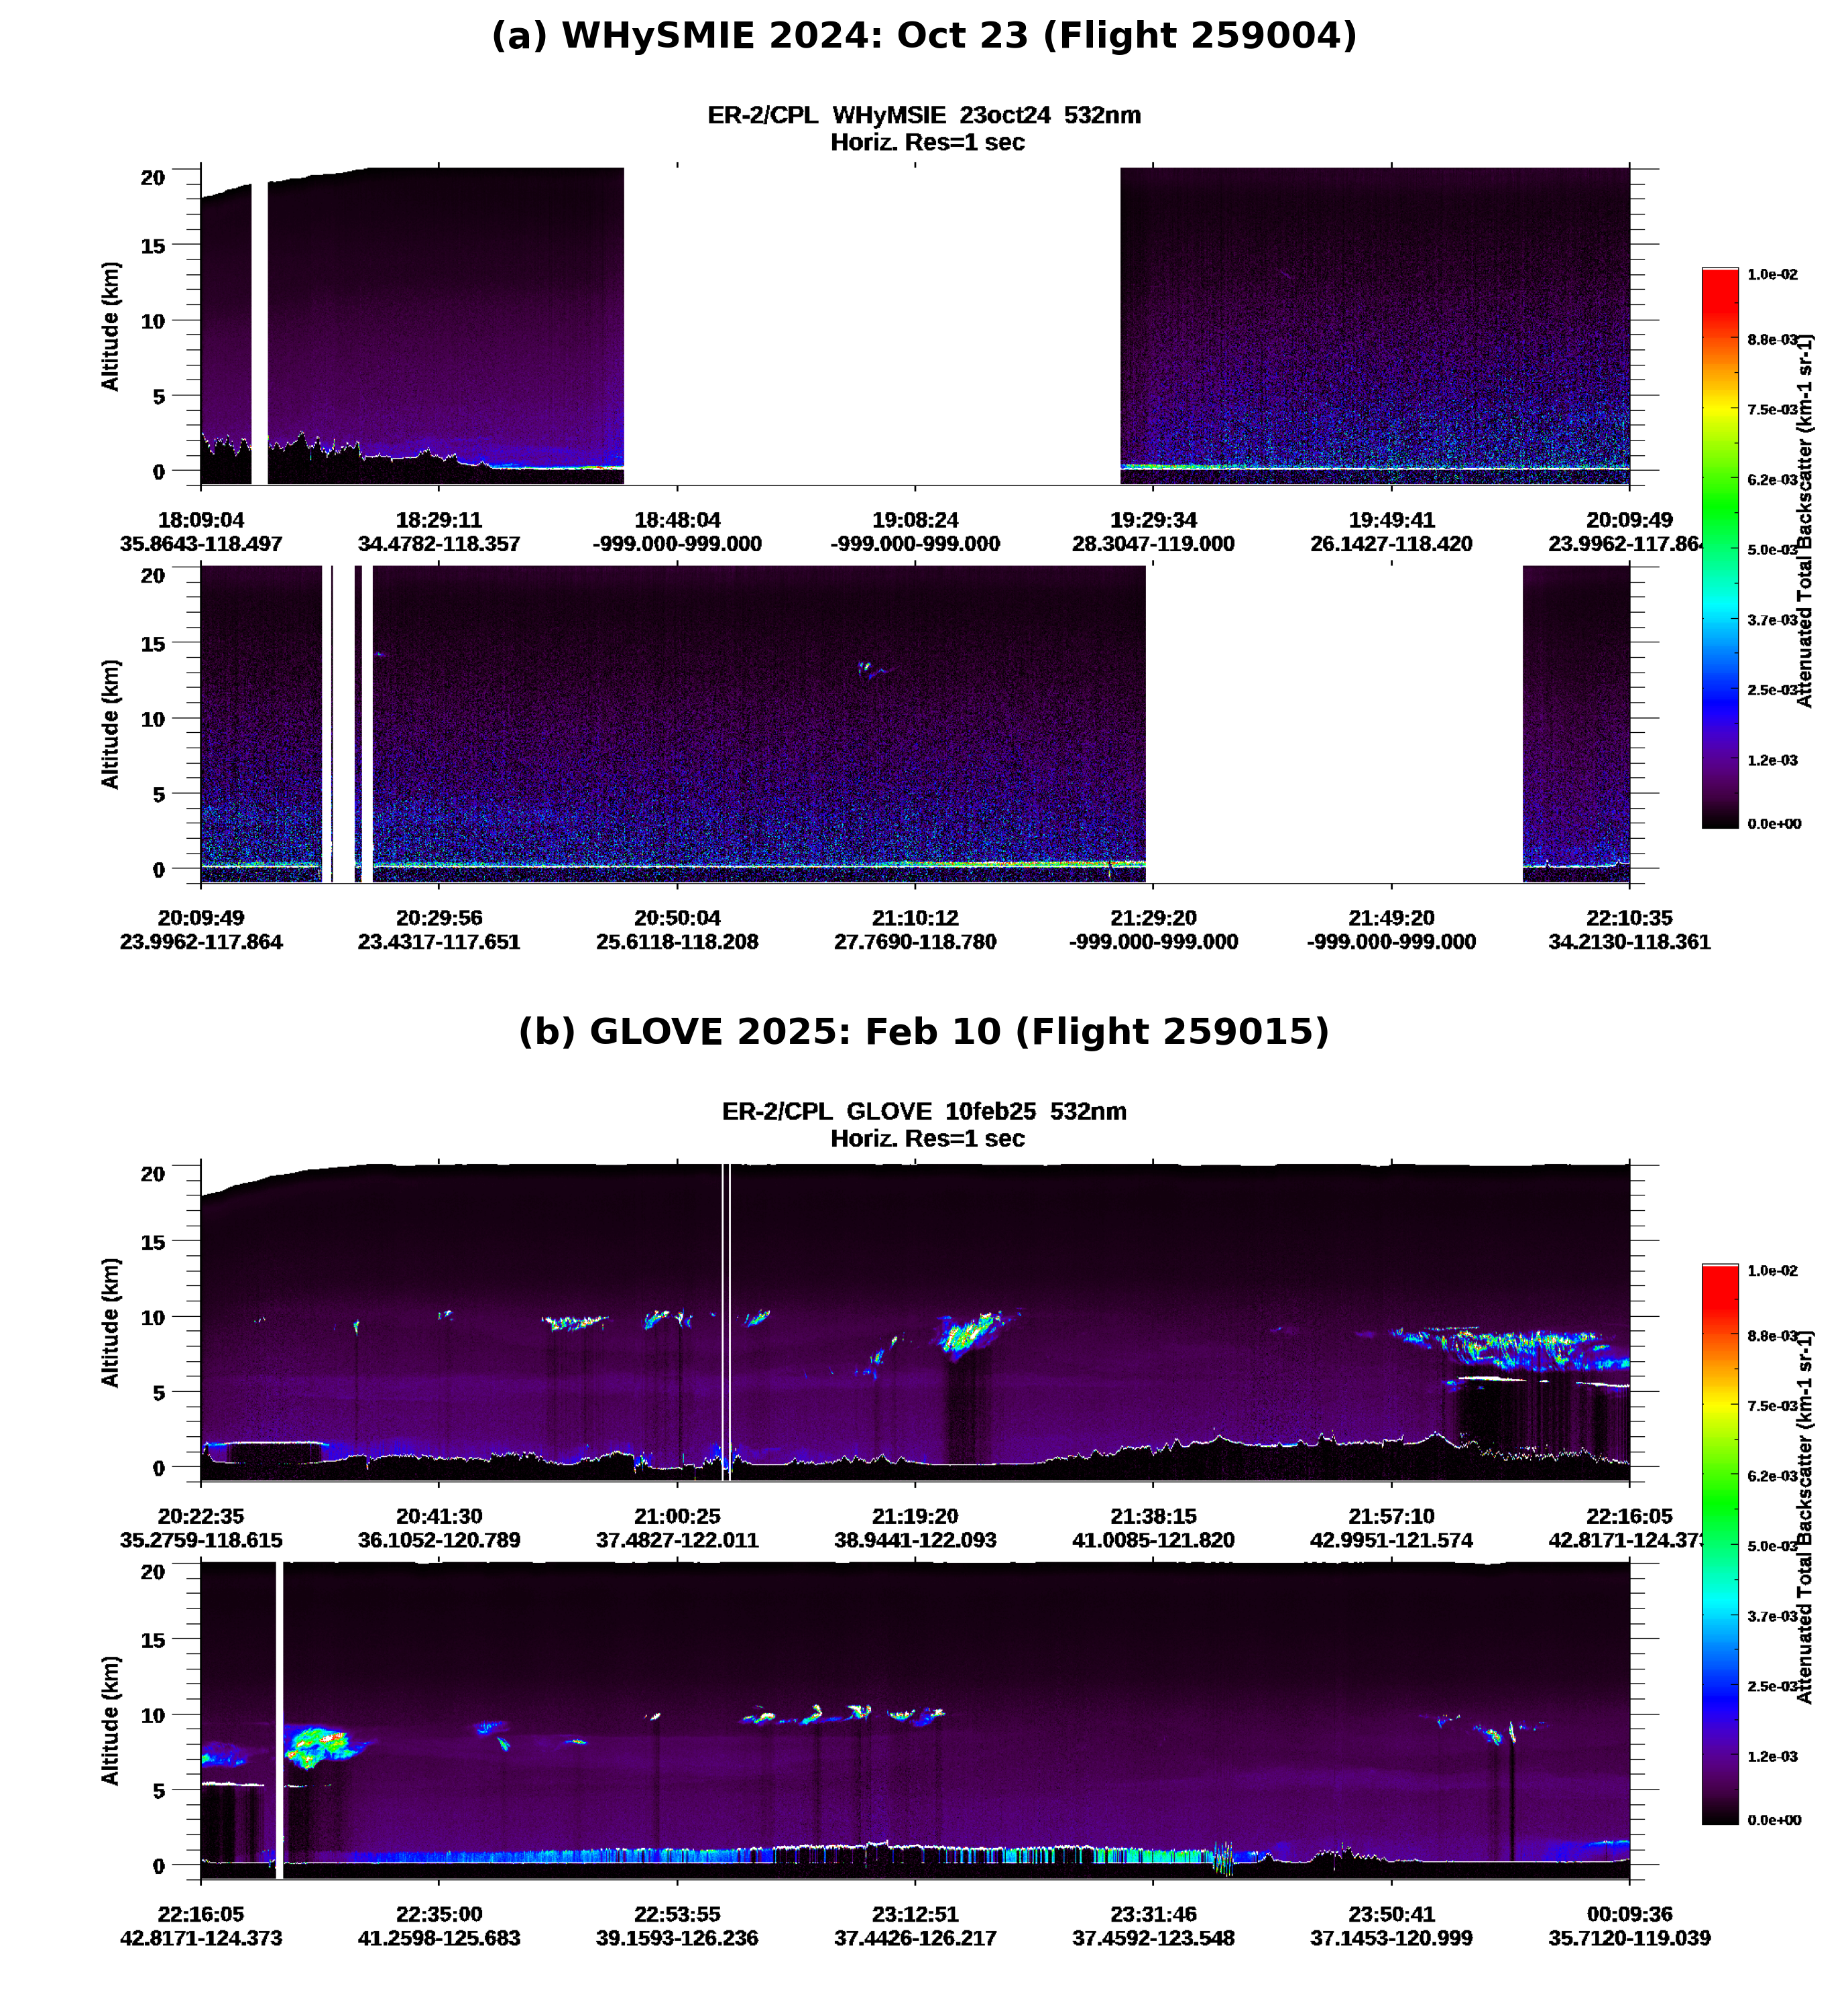
\includegraphics[width=0.95\textwidth]{paperfigures/paper2_fig1_domain_comparison_backscatter.png}
    \caption{Official CPL 532 nm attenuated total backscatter curtains from October 23, 2024 (WHySMIE, flight 259004) and February 10, 2025 (GLOVE, flight 259015). Each panel shows outbound and return legs at 1-second horizontal resolution, 0--20 km altitude. Note the fundamentally different cloud structure: WHySMIE shows shallow marine boundary layer clouds below $\sim$2 km, while GLOVE shows multi-layer clouds extending to $\sim$10 km with more complex vertical structure.}
    \label{fig:domain_comparison}
\end{figure}

\subsubsection{Leave-One-Flight-Out Validation}

Standard cross-validation (pooled K-fold) reports R$^2$ = -2.05, but even this is inflated relative to the true cross-flight performance. Leave-one-flight-out (LOFO) validation---training on all flights except one, testing on the held-out flight---reveals even more severe generalization failure:

\begin{table}[h]
    \centering
    \caption{Leave-one-flight-out cross-validation results across all six flights. Results from a single reproducible pipeline: CPL L2 ocean-only BL clouds ($\leq$ 2 km), nearest-hour ERA5 matching, 34 features, GBDT (200 trees).}
    \label{tab:lofo}
    \begin{tabular}{lccc}
        \toprule
        \textbf{Held-Out Flight} & \textbf{n\_test} & \textbf{R$^2$} & \textbf{MAE (m)} \\
        \midrule
        Oct 23, 2024 (WHySMIE) & 857 & -8.99 & 729 \\
        Oct 30, 2024 (WHySMIE) & 1808 & -0.61 & 633 \\
        Nov 4, 2024 (WHySMIE) & 1388 & -19.41 & 502 \\
        Feb 10, 2025 (GLOVE) & 608 & -1.97 & 543 \\
        Feb 12, 2025 (GLOVE) & 654 & -0.93 & 614 \\
        Feb 18, 2025 (GLOVE) & 185 & -0.26 & 86 \\
        \midrule
        \textbf{Mean} & -- & \textbf{-5.36} & \textbf{518} \\
        \bottomrule
    \end{tabular}
\end{table}

\textbf{Mean R$^2$ = -5.36} indicates predictions are substantially worse than a constant mean baseline. All six held-out flights produce negative R$^2$, with the most severe failure occurring on the Nov~4 WHySMIE flight (R$^2$ = -19.4, n=1388).

Figure~\ref{fig:cbh_distribution} shows the CBH distribution differences between flights that underlie this domain shift.

\begin{figure}[h]
    \centering
    \includegraphics[width=0.85\textwidth]{paperfigures/paper2_fig2_cbh_distribution_comparison.png}
    \caption{Cloud base height distributions for October 23, 2024 (WHySMIE, n=857 ocean-only, mean=138 m) and February 10, 2025 (GLOVE, n=608 ocean-only, mean=380 m) flights. Both distributions are right-skewed with a dominant low-CBH mode, but GLOVE shows a broader spread with secondary modes at 600--1400 m, reflecting its more complex multi-layer cloud structure.}
    \label{fig:cbh_distribution}
\end{figure}

\subsubsection{Understanding the Shift}

Kolmogorov-Smirnov (K-S) divergence quantifies feature distribution differences across flights:

\begin{table}[h]
    \centering
    \caption{K-S divergence for most shifted features (Oct 23 WHySMIE vs Feb 10 GLOVE). With 857 and 608 samples respectively, all p-values are effectively zero.}
    \label{tab:ks}
    \begin{tabular}{lcc}
        \toprule
        \textbf{Feature} & \textbf{K-S Statistic} & \textbf{p-value} \\
        \midrule
        t2m & 1.000 & <0.001 \\
        d2m & 1.000 & <0.001 \\
        blh & 1.000 & <0.001 \\
        t\_virtual & 1.000 & <0.001 \\
        moisture\_gradient & 1.000 & <0.001 \\
        theta\_e & 1.000 & <0.001 \\
        tcwv & 0.944 & <0.001 \\
        lcl & 0.954 & <0.001 \\
        stability\_index & 0.954 & <0.001 \\
        sp & 0.834 & <0.001 \\
        \bottomrule
    \end{tabular}
\end{table}

K-S statistics of 1.0 for key thermodynamic variables indicate completely non-overlapping distributions between the campaigns---a near-total shift in the feature space. Of the 34 features, 14 achieve the maximum K-S statistic of 1.0, and the lowest K-S statistic among base ERA5 variables is sp = 0.834. Only the solar angle features (sza\_cos, sza\_sin, saa\_cos, saa\_sin) show K-S = 0.0, since both campaigns operated at similar solar geometries. GLOVE 2025, conducted in February, flew northward along the California--Oregon coast and out over the northeast Pacific, sampling a marine environment with multi-layer cloud structures extending to $\sim$10 km. WHySMIE 2024, conducted in October, flew southward along the California--Baja California coast over the eastern Pacific, sampling a subtropical marine boundary layer environment with shallow clouds below $\sim$2 km. Despite both campaigns being primarily marine, the seasonal and latitudinal differences produce fundamentally different thermodynamic conditions.

PCA visualization confirms flights occupy non-overlapping regions of feature space (PC1 explains 36\% variance, separates campaigns).

Figure~\ref{fig:scatter_comparison} directly visualizes the domain shift through leave-one-out predictions.

\begin{figure}[h]
    \centering
    \includegraphics[width=0.95\textwidth]{paperfigures/paper2_fig3_scatter_comparison.png}
    \caption{Leave-one-flight-out scatter plots demonstrating domain shift. Left: October 23, 2024 (R$^2$ = -8.99, n = 857). Right: February 10, 2025 (R$^2$ = -1.97, n = 608). Both show predictions substantially worse than a constant baseline (red dotted line), consistent with the LOFO mean R$^2$ = -5.36 documented in Table~\ref{tab:lofo}.}
    \label{fig:scatter_comparison}
\end{figure}

\subsubsection{Why Standard CV Fails}

Temporal autocorrelation ($\rho$ = 0.94 at lag-1) means adjacent samples have nearly identical CBH values. When pooled K-fold CV splits consecutive samples across train/test folds, information leaks between folds. With 5,500 observations from six flights, pooled CV reports R$^2$ = -2.05 while LOFO reports R$^2$ = -5.36---both catastrophically negative, but the gap demonstrates that even pooled CV underestimates the severity of cross-regime failure.

\textbf{Lesson:} Always use temporally-aware validation for atmospheric time series. Pooled CV dramatically overestimates real-world performance.

Figure~\ref{fig:flight_comparison} shows the geographic context of both flights.

\begin{figure}[h]
    \centering
    \includegraphics[width=0.95\textwidth]{paperfigures/paper2_fig4_flight_path_comparison.png}
    \caption{Flight path comparison showing geographic context of domain shift. October 23, 2024 (WHySMIE, left) flew southward along the California--Baja coast over the eastern Pacific. February 10, 2025 (GLOVE, right) flew northward along the California--Oregon coast and out over the northeast Pacific. Colored points show ocean-only CBH observations used for analysis; gray points indicate over-land transit data that were excluded from the marine cloud study (WHySMIE: 106 excluded, GLOVE: 287 excluded).}
    \label{fig:flight_comparison}
\end{figure}

\subsection{Domain Adaptation Methods}

We evaluate five adaptation approaches:

\subsubsection{Few-Shot Learning (Most Effective)}

Fine-tune the base model on $k$ labeled samples from the target flight:

\begin{table}[h]
    \centering
    \caption{Few-shot adaptation performance (mean R$^2$ $\pm$ std across 20 random trials) by shot count.}
    \label{tab:fewshot}
    \begin{tabular}{lcccc}
        \toprule
        \textbf{Target Flight} & \textbf{5-shot} & \textbf{10-shot} & \textbf{20-shot} & \textbf{50-shot} \\
        \midrule
        Oct 23 (WHySMIE) & -1.06 & -0.09 & +0.29 & +0.40 \\
        Oct 30 (WHySMIE) & +0.37 & +0.55 & +0.60 & +0.69 \\
        Nov 4 (WHySMIE) & -2.73 & -1.40 & -0.38 & -0.03 \\
        Feb 10 (GLOVE) & -0.33 & +0.02 & +0.22 & +0.37 \\
        Feb 12 (GLOVE) & +0.03 & +0.21 & +0.43 & +0.59 \\
        Feb 18 (GLOVE) & -0.08 & -0.02 & +0.02 & +0.08 \\
        \midrule
        \textbf{Mean} & -0.63 & -0.12 & +0.20 & \textbf{+0.35} \\
        \bottomrule
    \end{tabular}
\end{table}

Few-shot learning recovers substantial performance with minimal labeling effort. With 50 samples, mean R$^2$ improves from -5.36 to +0.35.

\textbf{Variance across targets:} Oct 30 WHySMIE (closest to training distribution) recovers to R$^2$ = 0.69; Nov 4 WHySMIE (most different regime) only reaches R$^2$ = -0.03 even with 50 shots. Adaptation effectiveness depends on regime similarity.

\subsubsection{Instance Weighting (Failed)}

Reweight source samples to match target distribution using two approaches. The KNN-based method weights samples by distance to nearest target samples. The density ratio method estimates $p_{\text{target}}(x) / p_{\text{source}}(x)$ directly.

Results: Mean R$^2$ = -3.5 (KNN), -5.5 (density)---\textit{worse than or comparable to the LOFO baseline}.

\textbf{Why it fails:} No source samples are sufficiently similar to target regime. Reweighting amplifies noise without improving representation.

\subsubsection{TrAdaBoost (Marginal)}

Transfer learning via boosting that down-weights poorly-transferring source samples \cite{Dai2007}.

Result: Mean R$^2$ = +0.04, marginal improvement over baseline (-5.36), barely positive.

\subsubsection{MMD Feature Alignment (Failed)}

Project features to minimize Maximum Mean Discrepancy between source and target \cite{Long2015}.

Result: Mean R$^2$ = -7.9---\textit{worse than the LOFO baseline}. Alignment destroys predictive signal.

\textbf{Why it fails:} The features that differ most across domains (t2m, tcwv) are also most predictive. Aligning distributions removes the signal.

\subsubsection{Feature Selection (Marginal)}

Select features with lowest cross-domain divergence.

Result: Mean R$^2$ = -6.9, worse than the LOFO baseline. Selecting low-divergence features (primarily solar angles) removes the most predictive variables.

\subsection{Domain Adaptation Summary}

\begin{table}[h]
    \centering
    \caption{Domain adaptation method comparison (mean R$^2$ across 6 held-out flights).}
    \label{tab:adaptation_summary}
    \begin{tabular}{lcc}
        \toprule
        \textbf{Method} & \textbf{Mean R$^2$} & \textbf{Assessment} \\
        \midrule
        No adaptation (LOFO) & -5.36 & Baseline \\
        Instance weighting (KNN) & -3.5 & Marginal improvement \\
        Instance weighting (density) & -5.5 & Comparable to baseline \\
        MMD alignment & -7.9 & Worse \\
        Feature selection & -6.9 & Worse \\
        TrAdaBoost & +0.04 & Marginal positive \\
        \textbf{Few-shot (50 samples)} & \textbf{+0.35} & \textbf{Effective} \\
        \bottomrule
    \end{tabular}
\end{table}

\textbf{Recommendation:} For operational deployment to new atmospheric regimes, collect 20--50 labeled samples and fine-tune. Other adaptation methods fail for this application.

\section{Uncertainty Quantification}
\label{sec:uncertainty}

\subsection{Conformal Prediction Failure}

Split conformal prediction \cite{Lei2018} guarantees coverage under exchangeability. We evaluate on our atmospheric data:

\begin{table}[h]
    \centering
    \caption{Uncertainty quantification method comparison (cross-flight evaluation). Within-flight split conformal achieves 90.0\% coverage, but cross-flight evaluation degrades dramatically due to exchangeability violations.}
    \label{tab:uq}
    \begin{tabular}{lccc}
        \toprule
        \textbf{Method} & \textbf{Coverage} & \textbf{Target} & \textbf{Width (m)} \\
        \midrule
        Split conformal (cross-flight) & 34\% & 90\% & 557 \\
        \textbf{Per-flight calibration (within-flight)} & \textbf{90\%} & 90\% & 538 \\
        \bottomrule
    \end{tabular}
\end{table}

\textbf{Cross-flight split conformal achieves only 34\% coverage} (target: 90\%)---a catastrophic failure. In contrast, within-flight split conformal achieves 90.0\% coverage, confirming that the failure stems from exchangeability violations across flights rather than from the method itself.

\subsection{Why Conformal Fails}

Two exchangeability violations explain the coverage failure. The first is temporal autocorrelation, with $\rho$ = 0.94 at lag-1 indicating that adjacent samples have nearly identical CBH values. Calibration residuals from temporally-clustered data therefore underestimate test-time errors. The second violation is domain shift itself: when calibration data come from different flights than test data, residual distributions are non-representative of the true error distribution at deployment.

Adaptive conformal (which adjusts intervals based on local density) performs even worse (11\% coverage) because density estimation fails under distribution shift.

\subsection{Per-Flight Calibration}

We propose per-flight calibration: calibrate within each flight independently, evaluate on held-out portions of the same flight.

\begin{table}[h]
    \centering
    \caption{Within-flight conformal prediction results (split conformal, 90\% target).}
    \label{tab:perflight_uq}
    \begin{tabular}{lccc}
        \toprule
        \textbf{Flight} & \textbf{Coverage} & \textbf{Width (m)} & \textbf{R$^2$} \\
        \midrule
        Oct 23 (WHySMIE) & 89.5\% & 146 & 0.49 \\
        Oct 30 (WHySMIE) & 91.7\% & 956 & 0.83 \\
        Nov 4 (WHySMIE) & 89.9\% & 155 & 0.38 \\
        Feb 10 (GLOVE) & 89.3\% & 873 & 0.65 \\
        Feb 12 (GLOVE) & 93.1\% & 687 & 0.86 \\
        Feb 18 (GLOVE) & 86.5\% & 408 & -0.45 \\
        \midrule
        \textbf{Mean} & \textbf{90.0\%} & 538 & -- \\
        \bottomrule
    \end{tabular}
\end{table}

Per-flight calibration recovers 90.0\% coverage (matches 90\% target) by respecting the i.i.d. assumption within flights. Within-flight R$^2$ ranges from -0.45 (Feb~18, smallest flight with n=185) to 0.86 (Feb~12), demonstrating that prediction quality varies substantially across atmospheric regimes even within the same flight.

\textbf{Operational implication:} Conformal prediction cannot provide valid coverage guarantees across atmospheric regimes. Deploy per-flight calibration with locally-collected labeled samples.

\section{Discussion}
\label{sec:discussion}

\subsection{When This Approach Works}

The approach succeeds in several scenarios. Within-flight deployment with per-flight conformal calibration (60/20/20 train/cal/test split) achieves a mean R$^2$ across flights of 0.46 (ranging from -0.45 for the smallest flight to 0.86) with 90\% conformal coverage, demonstrating useful retrieval when training and test data share the same atmospheric regime. Note that full within-flight 5-fold CV yields a lower mean R$^2$ = -0.51 due to high variance across folds and flights, reflecting the difficulty of this regression task even within a single flight. Cross-regime deployment with few-shot adaptation recovers R$^2$ = -0.03--0.69 with only 50 labeled samples from the target domain, making operational deployment practical. Real-time inference at 0.28 ms on CPU makes the method suitable for aircraft deployment without specialized hardware.

\subsection{When This Approach Fails}

The approach fails in several important scenarios that practitioners must recognize. Cross-regime deployment without adaptation yields R$^2$ = -5.36, a catastrophic failure where predictions are substantially worse than a constant baseline. Even within-flight shuffled 5-fold CV yields mean R$^2$ = -0.51 across flights, indicating that GBDT struggles with this heterogeneous regression task. Conformal prediction under domain shift achieves only 34\% coverage versus the 90\% target, rendering uncertainty estimates unreliable. Instance weighting and MMD alignment not only fail to improve performance but actively make it worse or provide only marginal benefit.

\subsection{Practical Recommendations}

Based on our findings, we offer five practical recommendations for atmospheric ML practitioners. First, always use temporally-aware validation, as pooled CV reports R$^2$ = -2.05 while LOFO reveals the true cross-regime R$^2$ = -5.36; per-flight or time-ordered splits provide honest performance estimates. Second, expect domain shift, recognizing that high within-distribution performance does not guarantee cross-regime generalization; LOFO validation is essential before making deployment claims. Third, plan for few-shot adaptation by budgeting for collecting 20--50 labeled samples from each target regime, which is more practical than attempting universal models. Fourth, use per-flight uncertainty calibration, since standard conformal prediction fails under shift; calibrating locally within each deployment regime is necessary for reliable uncertainty estimates. Fifth, recognize that feature engineering aids interpretation rather than accuracy, as derived thermodynamic features reveal what physics matter but do not dramatically improve GBDT predictions since the algorithm learns equivalent representations from raw variables.

\subsection{Implications for Atmospheric ML}

Our findings challenge several assumptions common in atmospheric ML. First, cross-validation overstates generalization more severely than previously documented, with pooled CV (R$^2$ = -2.05) substantially overestimating performance relative to LOFO (R$^2$ = -5.36), and both being catastrophically negative. Second, physics-informed features provide limited accuracy gains, as GBDT with 5 raw ERA5 features achieves comparable pooled CV performance to the 34-feature enhanced model (both negative R$^2$), though the 34-feature model performs better in per-flight CV (R$^2$ = -0.51 vs -2.04), indicating that the value of feature engineering is context-dependent. Third, domain adaptation is harder than expected for atmospheric applications, with only few-shot learning proving effective while sophisticated methods including MMD and instance weighting fail. Fourth, uncertainty quantification requires particular care, as standard methods fail under the autocorrelation and shift inherent in atmospheric data.

\section{Conclusion}
\label{sec:conclusion}

We have presented a systematic investigation of physics-informed feature engineering and domain shift challenges for atmospheric machine learning. Five key findings emerge from this work. First, feature engineering provides interpretability benefits, with derived thermodynamic features revealing physically meaningful relationships, and modest per-flight accuracy improvements over base ERA5 variables (within-flight CV R$^2$ = -0.51 vs -2.04), though neither achieves positive R$^2$ across all flights. Second, domain shift is catastrophic for this application, with LOFO validation yielding R$^2$ = -5.36 across 5,500 ocean-only boundary-layer observations from six flights, representing among the most severe shifts documented in atmospheric ML literature. Third, few-shot learning is the only effective adaptation method, with 50 samples recovering mean R$^2$ = +0.35, while instance weighting, TrAdaBoost, and MMD alignment fail or provide only marginal benefit. Fourth, conformal prediction fails under shift, achieving only 34\% coverage versus the 90\% target, though within-flight calibration exactly recovers 90\% coverage. Fifth, honest expectations are essential: this approach works for within-regime deployment with local calibration but fails for universal cross-regime generalization.

We release our code, data, and trained models to support reproducible research on atmospheric ML generalization challenges.

\section*{Acknowledgments}

This work was conducted independently following the author's NASA OSTEM internship (May--August 2025). The author thanks the NASA Goddard Space Flight Center for data access during the internship period. ERA5 data were provided by ECMWF Copernicus Climate Data Store.

\section*{Code Availability}

All code, data processing pipelines, and trained models are available at \url{https://github.com/rylanmalarchick/CloudMLPublic} under MIT license.

\bibliographystyle{plain}
\begin{thebibliography}{25}

\bibitem[Dai et al.(2007)]{Dai2007}
Dai, W., Yang, Q., Xue, G.R., \& Yu, Y. (2007).
\newblock Boosting for transfer learning.
\newblock \textit{Proc. ICML}, 193--200.

\bibitem[Finn et al.(2017)]{Finn2017}
Finn, C., Abbeel, P., \& Levine, S. (2017).
\newblock Model-agnostic meta-learning for fast adaptation of deep networks.
\newblock \textit{Proc. ICML}, 1126--1135.

\bibitem[Ganin et al.(2016)]{Ganin2016}
Ganin, Y., et al. (2016).
\newblock Domain-adversarial training of neural networks.
\newblock \textit{J. Mach. Learn. Res.}, 17(1), 2096--2030.

\bibitem[Hersbach et al.(2020)]{Hersbach2020}
Hersbach, H., et al. (2020).
\newblock The ERA5 global reanalysis.
\newblock \textit{Q. J. R. Meteorol. Soc.}, 146(730), 1999--2049.

\bibitem[Lawrence(2005)]{Lawrence2005}
Lawrence, M.G. (2005).
\newblock The relationship between relative humidity and the dewpoint temperature in moist air.
\newblock \textit{Bull. Am. Meteorol. Soc.}, 86(2), 225--233.

\bibitem[Lei et al.(2018)]{Lei2018}
Lei, J., G'Sell, M., Rinaldo, A., Tibshirani, R.J., \& Wasserman, L. (2018).
\newblock Distribution-free predictive inference for regression.
\newblock \textit{J. Am. Stat. Assoc.}, 113(523), 1094--1111.

\bibitem[Long et al.(2015)]{Long2015}
Long, M., Cao, Y., Wang, J., \& Jordan, M. (2015).
\newblock Learning transferable features with deep adaptation networks.
\newblock \textit{Proc. ICML}, 97--105.

\bibitem[Rasp \& Lerch(2018)]{Rasp2020}
Rasp, S., \& Lerch, S. (2018).
\newblock Neural networks for post-processing ensemble weather forecasts.
\newblock \textit{Mon. Weather Rev.}, 146(11), 3885--3900.

\bibitem[Shafer \& Vovk(2008)]{Shafer2008}
Shafer, G., \& Vovk, V. (2008).
\newblock A tutorial on conformal prediction.
\newblock \textit{J. Mach. Learn. Res.}, 9, 371--421.

\bibitem[Shimodaira(2000)]{Shimodaira2000}
Shimodaira, H. (2000).
\newblock Improving predictive inference under covariate shift.
\newblock \textit{J. Stat. Plan. Inference}, 90(2), 227--244.

\bibitem[Stubenrauch et al.(2021)]{Stubenrauch2021}
Stubenrauch, C.J., et al. (2021).
\newblock Reanalysis cloud property retrievals.
\newblock \textit{J. Geophys. Res. Atmos.}, 126, e2020JD033717.

\bibitem[Tuia et al.(2016)]{Tuia2016}
Tuia, D., et al. (2016).
\newblock Domain adaptation for the classification of remote sensing data.
\newblock \textit{IEEE Geosci. Remote Sens. Mag.}, 4(2), 7--28.

\end{thebibliography}

\end{document}
